\documentclass[journal=jcisd8,manuscript=article]{achemso}
\SectionNumbersOn

\usepackage{microtype}
\usepackage{graphicx}
\usepackage{float}
\usepackage{subcaption}
\usepackage{booktabs}
\usepackage{amsmath}
\usepackage{amssymb}
\usepackage{mathtools}
\usepackage{amsthm}
\usepackage{url}
\usepackage{enumitem}
\usepackage{tabularx}
\usepackage{siunitx}
\sisetup{range-phrase=--,range-units=single}
\usepackage{xcolor}
\usepackage[most]{tcolorbox}
\usepackage{caption}
\usepackage{verbatim}
\usepackage{hyperref}
\usepackage[capitalize,noabbrev]{cleveref}

\newif\ifrevision
\revisiontrue
\providecommand{\textalpha}{\ensuremath{\alpha}}

\ifrevision
  \newcommand{\new}[1]{\textcolor{blue}{#1}}
  \newcommand{\newtable}{\color{blue}}
\else
  \newcommand{\new}[1]{#1}
  \newcommand{\newtable}{}
\fi

\newtcolorbox{userbox}{
  colback=blue!5!white,
  colframe=blue!20!white,
  boxsep=5pt,
  arc=4mm,
  left=10pt,
  right=10pt,
  top=10pt,
  bottom=10pt,
  breakable,
}

\newtcolorbox{assistantbox}{
  colback=black!5!white,
  colframe=black!20!white,
  boxsep=5pt,
  arc=4mm,
  left=10pt,
  right=10pt,
  top=10pt,
  bottom=10pt,
  breakable,
}
\author{Carles Navarro}
\email{c.navarro@acellera.com}
\affiliation[Acellera Labs]{Acellera Labs, C/ Doctor Trueta 183, 08005 Barcelona, Spain}
\alsoaffiliation[Universitat Pompeu Fabra]{Computational Science Laboratory, Universitat Pompeu Fabra, PRBB, C/ Doctor Aiguader 88, 08003 Barcelona, Spain}

\author{Mariona Torrens}
\affiliation[Acellera Labs]{Acellera Labs, C/ Doctor Trueta 183, 08005 Barcelona, Spain}

\author{Philipp Tholke}
\affiliation[Acellera Labs]{Acellera Labs, C/ Doctor Trueta 183, 08005 Barcelona, Spain}

\author{Stefan Doerr}
\affiliation[Acellera Labs]{Acellera Labs, C/ Doctor Trueta 183, 08005 Barcelona, Spain}

\author{Gianni de Fabritiis}
\email{g.defabritiis@acellera.com}
\affiliation[Acellera Labs]{Acellera Labs, C/ Doctor Trueta 183, 08005 Barcelona, Spain}
\alsoaffiliation[Universitat Pompeu Fabra]{Computational Science Laboratory, Universitat Pompeu Fabra, PRBB, C/ Doctor Aiguader 88, 08003 Barcelona, Spain}
\alsoaffiliation[ICREA]{Instituci\'{o} Catalana de Recerca i Estudis Avan\c{c}ats (ICREA), Passeig Llu\'{i}s Companys 23, 08010 Barcelona, Spain}

\title[Speak to a Protein: An Interactive Multimodal Co-Scientist]{Speak to a Protein: An Interactive Multimodal Co-Scientist for Protein Analysis}
\keywords{Agentic co-scientist, scientific discovery, molecular visualization, deep research, drug discovery, retrieval-augmented generation}

\begin{document}

\begin{abstract}
Building a working mental model of a protein typically requires weeks of reading, cross-referencing crystal and predicted structures, and inspecting ligand complexes, an effort that is slow, unevenly accessible, and often requires specialized computational skills. We introduce \emph{Speak to a Protein}, a new capability that turns protein analysis into an interactive, multimodal dialogue with an expert co-scientist. The AI system retrieves and synthesizes relevant literature, structures, and ligand data; grounds answers in a live 3D scene; and can highlight, annotate, manipulate and see the visualization. It also generates and runs code when needed, explaining results in both text and graphics.
We demonstrate these capabilities on relevant proteins, posing questions about binding pockets, conformational changes, or structure-activity relationships to test ideas in real-time. \emph{Speak to a Protein} reduces the time from question to evidence, lowers the barrier to advanced structural analysis, and enables hypothesis generation by tightly coupling language, code, and 3D structures. 
Speak to a Protein is freely accessible at \url{(URL to be disclosed after publication)}.

\end{abstract}

\section{Introduction}\label{sec:intro}
Proteins are the molecular machinery of life, and understanding their structure and function is fundamental to modern biology and medicine. For a researcher in drug discovery or molecular biology, developing an intuitive, "working mental model" of a target protein, its active sites, its conformational dynamics, and its network of interactions is a critical first step. However, this process is slow and arduous, often requiring a combination of deep domain knowledge and specialized computational skills.

A researcher investigating a protein kinase to understand how a new series of inhibitors might bind must embark on a fragmented and technically demanding workflow. This involves sifting through the PubMed literature~\citep{Sayers2020}, fetching and comparing multiple structures from the Protein Data Bank (PDB)~\citep{Burley2018}, querying UniProt~\citep{UniProt2022}  for functional annotations and disease-associated variants, and extracting structure-activity relationship (SAR) data from databases like ChEMBL~\citep{Mendez2018}. Each step requires navigating different interfaces and data formats. Furthermore, deeper analysis, such as superimposing structures, identifying key interactions, or plotting bioactivity data, requires proficiency with specialized software or scripting languages, creating a significant barrier to entry for many bench scientists. This high friction for asking and answering questions restrains curiosity and slows the pace of discovery.

To address these challenges, we introduce \emph{Speak to a Protein}, a new capability designed to transform protein analysis into an interactive dialogue with an AI co-scientist that collaborates with the user in real-time. Using recent advances in large language models (LLMs) and their evolution into multimodal scientific agents \citep{Caffagni2024, Zhang2024, Zheng2025}, our system can comprehend complex, natural language queries about a protein of interest. It autonomously retrieves, integrates, and synthesizes information from a comprehensive suite of biological data sources, including literature, structural repositories, and biochemical databases.

The core innovation of \emph{Speak to a Protein} is its ability to ground its responses across multiple, synchronized modalities. When a user asks a question, the AI does not simply return text. It interacts with a live 3D structural viewer to highlight residues, measure distances, or annotate binding pockets. It can generate and execute code in a sandboxed environment to perform calculations, filter tabular data, or generate plots on the fly. Furthermore, the AI co-scientist sees, understands and controls the visualization, offering a natural interaction with the user. This tight coupling of natural language, 3D visualization, and code execution creates a seamless and intuitive environment for scientific exploration.

This paper makes the following contributions: We present the design and architecture of an AI system that integrates language, code execution, and 3D visualization for interactive protein analysis. We show how this multimodal approach drastically lowers the barrier to complex structural and biochemical data analysis. Through case studies on relevant proteins and benchmarks, we show that this system enables a more fluid and powerful form of hypothesis generation, accelerating the cycle from question to evidence.

\section{Related Work}\label{sec:related}
%AI Scientist
The ambition to create an AI capable of scientific discovery is a long-standing goal, articulated in visions such as Hiroaki Kitano's proposal for an "AI Scientist": a system that could autonomously formulate hypotheses, design experiments, and achieve Nobel-class discoveries \citep{kitano2021}. Recent systems push this frontier further: \emph{Kosmos} \citep{mitchener2025kosmos} runs multi-hour autonomous campaigns that read thousands of papers and execute tens of thousands of lines of analysis code per task. While such fully autonomous systems \citep{boiko2023autonomous, zou2025agente, mitchener2025kosmos} remain a grand challenge, recent progress in large language models (LLMs) has enabled the development of a more immediate and collaborative paradigm: the "AI co-scientist" \citep{gottweis2025coscientist} or "advanced intelligence" in Kitano's words.

%\subsection{Conversational and Multimodal Protein Assistants}
Early systems explored conversational interfaces for structural inspection and Q\&A over proteins. \citet{guo2023proteinchat} demonstrated \emph{ProteinChat}, which couples LLM prompting with protein 3D structures to answer user questions about residues and pockets. Contemporary efforts such as \citet{wang2024protchatgpt} and \citet{xiao2024proteingpt} investigate protein-aware prompting and multimodal conditioning for function/property reasoning. Most recently, \citet{wang2025prot2chat} proposes \emph{Prot2Chat}, an LLM that fuses protein sequence, structure, and text via an early-fusion adapter, directly targeting protein Q\&A. Complementary work strengthens the protein side itself, with structure-enhanced instruction tuning \citep{wu2025sepit} and trimodal alignment of sequence, structure, and language for advanced protein search \citep{su2025protrek}.

%\subsection{Structure-Aware Tools and Visualization Copilots}
Beyond text-only chat, domain copilots increasingly drive molecular viewers and modeling tools. \citet{sun2024chatmol} introduce \emph{ChatMol Copilot}, an LLM agent that coordinates cheminformatics and modeling tools (e.g., docking, conformer generation) in response to natural-language requests. In parallel, \citet{ille2024gpt4structural} systematically evaluates GPT-4's ability to perform rudimentary structural modeling and protein–ligand interaction analysis, highlighting both promise and limitations. Our work is aligned with this line but centers on tightly coupling language, code execution, and a live 3D scene for grounded, interactive answers.

%\subsection{Agentic LLMs for Chemistry and Drug Discovery}
Agent frameworks augment LLMs with tool use, retrieval, and planning. \emph{ChemCrow} \citep{bran2024chemcrow} shows that equipping GPT-4 with chemistry tools enables multi-step synthesis planning and materials tasks. More recently, CLADD \citep{lee2025cladd} proposes a retrieval-augmented multi-agent system specialized for drug discovery tasks. Multi-agent platforms extend this paradigm to end-to-end workflows: \emph{LLM-RDF} \citep{ruan2024llmrdf} coordinates six specialized agents across literature scouting, experiment design, hardware execution, and result interpretation, while \emph{ChatInvent} \citep{he2026chatinvent} brings agentic molecular design and synthesis planning into a real-world pharmaceutical setting. At broader scope, \emph{Biomni} \citep{huang2025biomni} pairs LLM reasoning with retrieval-augmented planning and code execution over a large catalogue of biomedical tools and databases, targeting general-purpose biomedical workflows. \emph{Speak to a Protein} adopts the agentic paradigm for structural biology: it retrieves literature/structures, executes analyses, and grounds responses in synchronized 3D visualizations.

\section{System Overview: \emph{Speak to a Protein}}\label{sec:overview}

\subsection{Architecture}

The system architecture of \emph{Speak to a Protein} (\cref{fig:architecture}) is organized around four components: a frontend with a chat panel and a 3D viewer where the user and the agent inspect and manipulate structures for 3D reasoning, an agent harness that runs the agent loop and exposes tools to the language model, a search service that maintains semantic indices over codebases, documentation, and literature, and a sandboxed filesystem in which the agent runs code against a preinstalled scientific software stack.

\begin{figure}[H]
\centering

\includegraphics[width=\textwidth]{Figures/architecture.png}
\caption{\textbf{Overview of the system architecture.} The Frontend hosts a chat panel, a 3D molecular viewer, and an IPython console. The Agent Harness runs the agent loop, holds conversation memory, and executes tool calls. A search service indexes codebases, documentation, and literature. A sandboxed filesystem provides a per-project workspace and a preinstalled scientific software stack, with restricted network egress.}\label{fig:architecture}
\end{figure}

The frontend hosts the chat panel, the 3D molecular viewer (\cref{fig:viewer} and \cref{subsec:viewer}), and a Pyodide-based IPython console for client-side analysis. The user converses through the chat panel; the frontend renders the agent's text replies and applies viewer commands as the agent issues them.

At each user request, the agent harness drives an agent loop: the model emits tool calls, the harness dispatches them, and their outputs are fed back into the next model invocation, continuing until the task is complete. To handle long sessions, the memory module autocompacts older turns into a working memory: a compact, adaptive summary that the agent itself rewrites at each compaction and that is reinjected into context on subsequent turns.


\subsection{Tools}\label{sec:tools}

The system exposes several tools to the agent, a set of core primitives that run code and edit files inside the sandbox, viewer tools that drive the 3D viewer in the frontend, a semantic search service over indexed library codebases, and a literature retrieval tool that gathers relevant publications for a given protein.

\noindent\textbf{Core tools.} The system's core tools are a set of primitives that execute shell commands in the sandbox, read, write, and edit files there, visualize images, read PDFs, and delegate self-contained subtasks to sub-agents. All execution happens inside the sandboxed filesystem of \cref{fig:architecture}, a Docker container with a per-session project workspace, a preinstalled scientific software stack, and outbound network restricted by a forward proxy that allowlists scientific domains. The stack spans Python, R with Bioconductor, and command-line bioinformatics tools. Files persist across turns, supporting iterative refinement and reproducibility.

\noindent\textbf{Viewer Tools.} The viewer tools provide the functionality to load project files into the viewer, execute code in the viewer's IPython session for visualization control and structural manipulation, capture screenshots of the rendered state, and save modified objects back to the project workspace. The bridge between the harness and the viewer is a session-bound WebSocket, each chat holds a single persistent channel. Screenshots are returned to the agent automatically after most viewer operations, providing a vision channel for grounding subsequent reasoning.


\noindent\textbf{Codebase Search.} The codebase search service holds vector indices over library codebases and their documentation, including MoleculeKit and HTMD \citep{Doerr2016}. This provides the agent with a fast semantic search over the codebase to inspect and discover how to use these scientific packages.

\noindent\textbf{Literature Search.}\label{sec:data:literature} The literature tool assembles a protein-conditioned RAG corpus on demand. While the corpus is built from \emph{curated references from UniProt}, it accepts a UniProt accession, a PDB identifier, or a FASTA sequence; each is resolved to a set of UniProt entries (a PDB code maps through its cross-references, a FASTA sequence is matched against PDB structures and then to UniProt), and the references listed under those entries form the corpus. Open-access articles are fetched from PubMed Central and indexed with LlamaIndex~\citep{Liu_LlamaIndex_2022} into a per-protein vector store cached on disk and keyed on the FASTA hash (Table~S1). At query time the agent issues a free-text query and receives the top-$k$ relevant passages with their citations. Index construction completes in one to two minutes for a new protein; subsequent queries on the same target are served from cache in seconds.


\subsection{Scientific Skills}\label{sec:skills}

\emph{Skills} are documentation packages that teach the agent how to use a particular database, library, or workflow~\citep{anthropic_skills_2025}. Each skill describes the relevant inputs and identifiers, the APIs to call, and idiomatic usage patterns, and may bundle example scripts the agent can adapt. Skills are exposed through progressive disclosure: at session start the agent receives only a one-line summary of every available skill, and reads the full body when one becomes relevant.

We currently provide skills for protein and structure databases (UniProt, PDB, AlphaFoldDB), chemical and bioactivity databases (ChEMBL, PubChem, DrugBank, ZINC), gene and genomic databases (NCBI Gene, Ensembl), and biomedical literature retrieval (PubMed). New databases or workflows are added by authoring a new skill, without modifying the core system.



\subsection{Agentic 3D Grounding and Interfaces with Scientists}\label{subsec:viewer}

Understanding proteins requires the navigation of multiple types of information, such as three-dimensional structures, experimental assay tables, and textual annotations. A central goal of \emph{Speak to a Protein} is to connect these diverse modalities through a single conversational interface, ensuring that system responses are not only generated in natural language but are also grounded in concrete evidence such as 3D visualizations, data tables, and executable code. This grounding operates bidirectionally: users can visually verify AI-generated hypotheses, while the AI agent itself can capture and interpret viewer states to inform its reasoning. To achieve this, we provide a set of interactive interfaces that extend dialogue into complementary domains: a structural viewer for molecular inspection, a tabular analysis environment for filtering and plotting assay data, and mechanisms for synchronizing actions across views. Together, these interfaces enable users to fluidly transition between asking questions, running analyses, and visually verifying hypotheses. Significantly, we are building these capabilities on top of a web application that has already attracted more than 18,000 registered users over the years, even in the absence of these AI features. These new capabilities enable medicinal chemists with no-code experience to use the tools like an expert computational chemist. We thus anticipate that it will be used by a considerable number of scientists, as demonstrated by the platform usage metrics in Appendix~S1.3.


In \emph{Speak to a Protein}, these functionalities are built using an entirely client-side sandbox for dynamic visualization and manipulation of molecular structures \citep{torrens2023playmolecule}. The sandbox builds on a browser-based molecular visualization toolkit that combines the high-performance \texttt{mol*} visualization engine \citep{Sehnal2021},  capable of rendering large biomolecular structures and molecular dynamics trajectories directly in the browser, with a WebAssembly-enabled Python runtime (Pyodide). This allows the use of powerful Python libraries such as MoleculeKit \citep{Doerr2016} in the client environment, enhancing the viewer's capabilities to load and manipulate a wide range of common structural file formats, from PDB and CIF to molecular dynamics trajectory files such as XTC and TRR.


\begin{figure}[H]
\centering
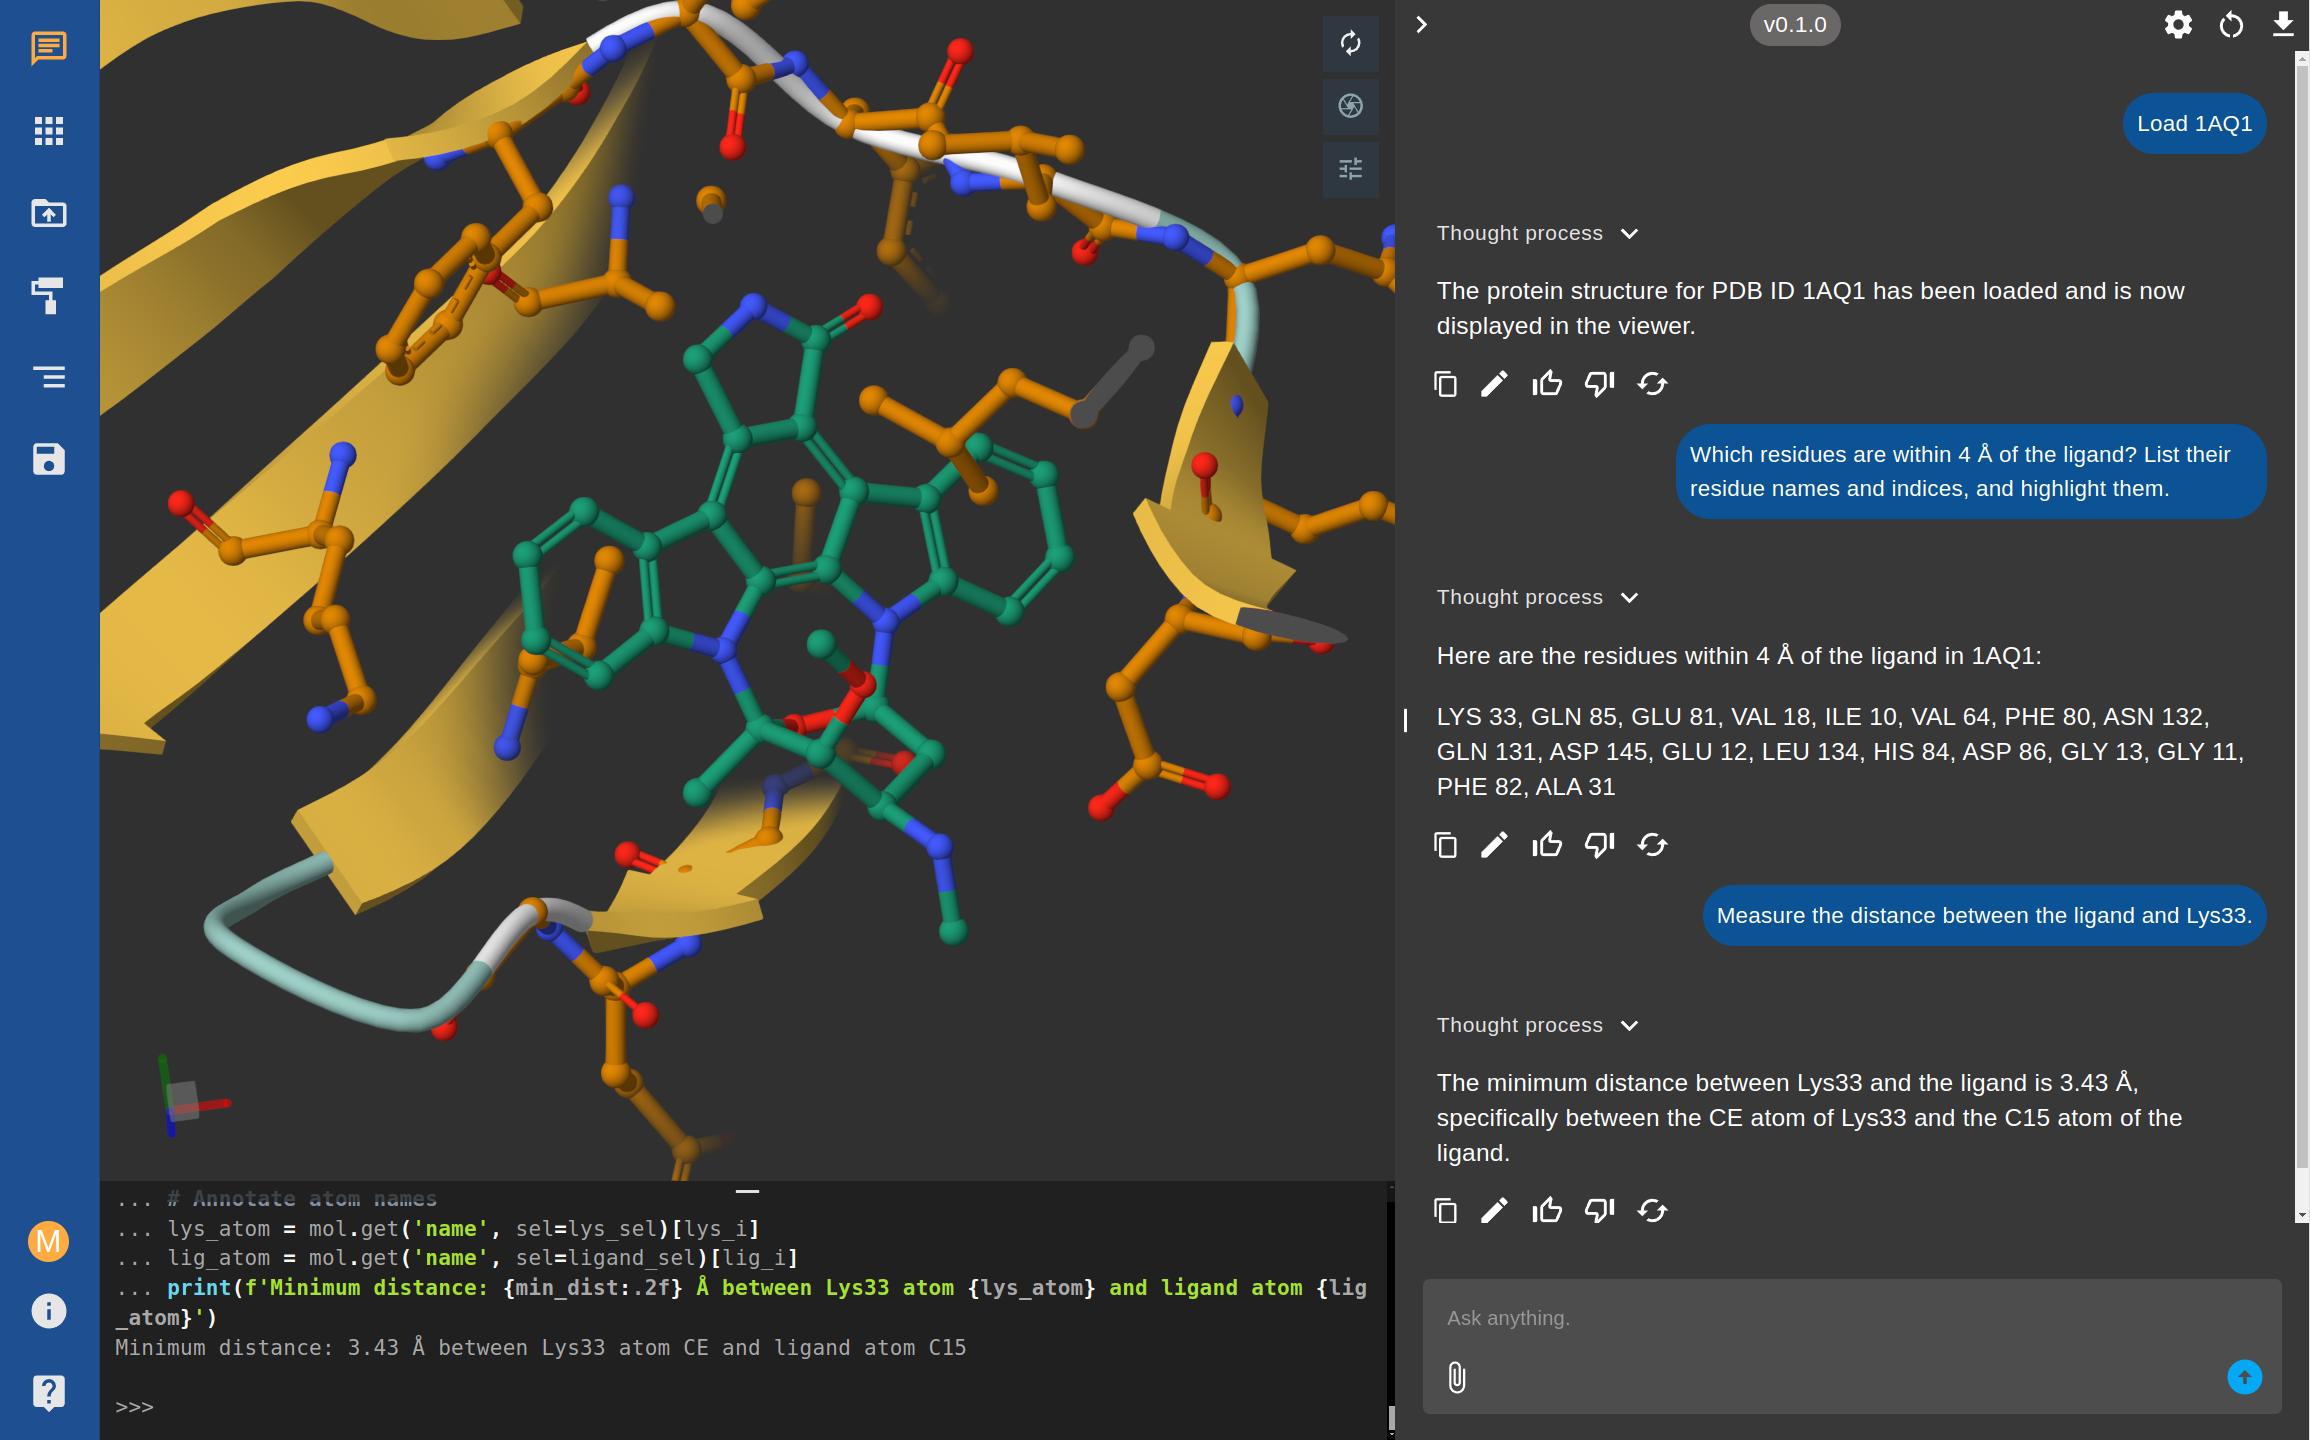
\includegraphics[width=\columnwidth]{Figures/viewer.png}
\caption{
    \textbf{Interactive analysis of the CDK2 structure (PDB: 1AQ1) using the \emph{Speak to a Protein} multimodal assistant.}
    The user enters natural language queries in the chat panel (right), and the system responds with both textual answers and real-time updates to the 3D visualization (left). Python code executed in the integrated sandbox is shown in the console (bottom), providing full transparency and reproducibility of the underlying analyses.
}\label{fig:viewer}
\end{figure}

A key feature is the ability to control this viewer through natural language commands. Requests such as "highlight the ATP-binding site" are translated into tool calls that execute Python code within the viewer, producing visual changes in real time (\cref{fig:viewer}). Beyond user-initiated actions, the agent can autonomously capture screenshots of the current viewer state and analyze them using vision capabilities. This agentic 3D vision enables the model to verify the results of its own manipulations, identify structural features that may not be explicitly encoded in the data, and iteratively refine visualizations based on what it observes. 

%Users can request a broad set of actions, such as:
%\begin{itemize}[leftmargin=1em]
%    \item \textbf{Loading structures}: Users can instruct the system to load structures either from public sources or by uploading custom files.
%    \item \textbf{Controlling the visualization}: The AI can create, modify, or remove molecular representations on demand. Structures or any of their subsets can be rendered in diverse styles, such as cartoon, ball-and-stick, spacefill, or surface, and colored according to different properties, such as chain, residue type, secondary structure, or user-defined colors. The selection logic uses the expressive VMD selection language, enabling complex queries like "show only the protein backbone," "highlight tyrosine residues in chain A," or "display all residues within 5~\AA{} of the ligand."
%    \item \textbf{Focusing the viewer}: The camera can be centered or zoomed onto regions of interest, such as active sites, mutated residues, or selected domains.
%    \item \textbf{Performing measurements}: Users can request measurements of distances, angles, or dihedrals between atoms or residues.
%    \item \textbf{Manipulating structures}: The system can modify loaded structures, for example, by filtering out water molecules or other unwanted components, splitting chains, or extracting subsets for closer inspection.
%    \item \textbf{Structural alignment}: Multiple structures can be superimposed based on selected atoms (e.g., C$\alpha$ atoms), allowing direct comparison of conformational states or homologous proteins.

%\end{itemize}



%\subsection{Tabular Data Analysis: Filtering, Analytics, Plots}


\section{Experiments}\label{sec:cases}
Evaluating agentic systems for computational biology is challenging: most existing benchmarks probe isolated capabilities rather than integrated, multi-step scientific work. We assess \emph{Speak to a Protein} on \emph{BixBench-Verified-50} \citep{phylo2026bixbenchverified} and complement the benchmark with two case studies on the dopamine D3 receptor (D3R) \citep{Chien2010} and cyclin-dependent kinase 2 (CDK2) \citep{Malumbres2009}, which illustrate how the system integrates data from multiple sources, generates insights through interactive multi-modal analysis, and produces a structured structured LaTeX report that can be shared and queried later. All experiments use GPT-5.4 as the foundational language model driving the agent.

\subsection{BixBench-Verified-50}\label{subsec:bixbench}
\emph{BixBench} \citep{mitchener2025bixbench} comprises real-world computational biology scenarios with open-answer questions covering data exploration, multi-step analytical workflows, and interpretation of nuanced results. Frontier models on the original benchmark scored near 17\% in the open-answer regime, exposing both genuine agent limitations and substantial benchmark noise. \emph{BixBench-Verified-50} \citep{phylo2026bixbenchverified} is a 50-task curated subset in which domain experts removed or rewrote ambiguous items and corrected faulty ground truths, isolating actual agent capability.

BixBench-Verified-50 emphasises bioinformatics analysis tasks (sequencing, single-cell, statistical genomics) that partially overlap with the structural biology workflows \emph{Speak to a Protein} primarily targets, motivating the complementary case studies that follow. On this benchmark \emph{Speak to a Protein} reached \textbf{78.5\%} accuracy, surpassing strong general-purpose coding agents such as Claude Code with Opus 4.6 (65.3\%) and the OpenAI Agents SDK with GPT-5.2 (61.3\%), and matching Edison Analysis at 78.0\% (\cref{fig:bixbench}). The leading score is held by Biomni Lab \citep{huang2025biomni} at 88.7\%, a system whose tool catalogue and curated retrieval corpus are explicitly tuned for the bioinformatics workflows that dominate this benchmark. We read the result as encouraging: \emph{Speak to a Protein}'s agentic substrate transfers well outside its structural biology focus, while the remaining gap to a domain-tuned bioinformatics agent confirms the value of specialised tooling for specialised tasks.

\begin{figure}[H]
\centering
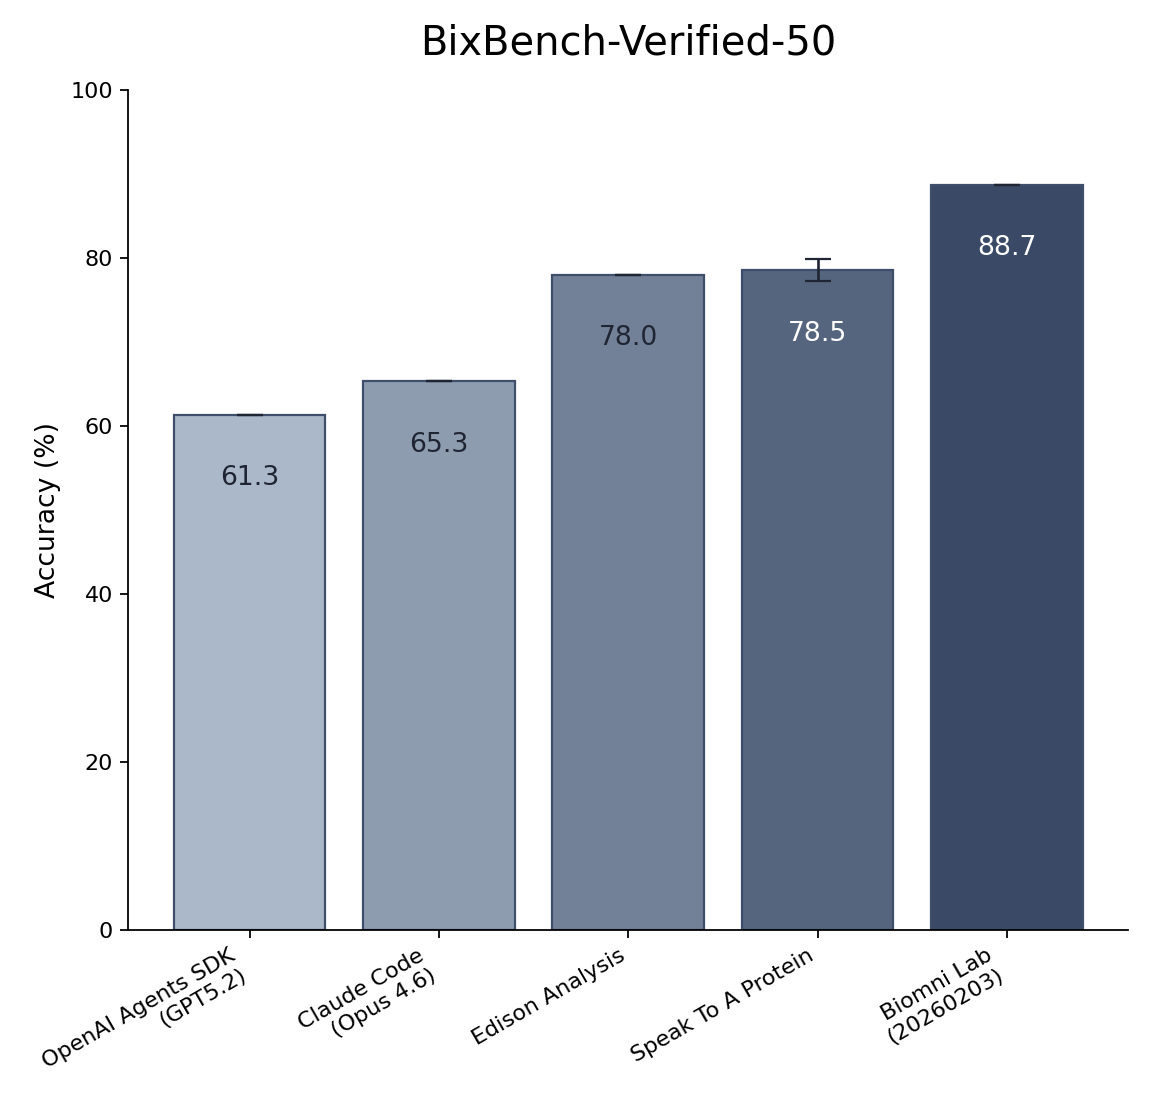
\includegraphics[width=0.85\columnwidth]{Figures/bixbench_verified_stap.png}
\caption{Accuracy on BixBench-Verified-50. Baseline scores are reproduced from the public leaderboard; error bars for \emph{Speak to a Protein} indicate variability across repeated runs.}
\label{fig:bixbench}
\end{figure}

\subsection{Speaking about the Dopamine D3 receptor (D3R)}
We use \emph{Speak to a Protein} to address a series of research questions related to D3R,  a G protein-coupled receptor of significant pharmacological interest.
In the video trace \url{https://youtu.be/H6ag4JJAM0w}, we show a possible user interaction with our system centered on D3R. The user begins by asking about the available structures for this receptor, loading the listed structure 3PBL. Next, the user instructs the system to filter for chain A, and changes the visual representation to focus on the binding pocket. Finally, it requests a list of known inhibitors associated with D3R. All this information is collected and made available to the AI so that knowledge is gathered and contextualized.

Focusing on the last query, we illustrate the workflow of the system (\cref{fig:d3r-table}). Upon the user's request, the AI used several tools in sequence to produce the necessary data. Using these tools, it identified the correct UniProt entry for D3R and used it to query ChEMBL for all relevant bioactivity data. The retrieved assay results were compiled and automatically stored in a CSV file, which was then loaded directly into the viewer for exploration and analysis.
The resulting table provides an overview of all known D3R inhibitors, along with chemical structures, assay details, potency metrics (such as EC${50},IC{50},K_i$), and references to the corresponding literature. Notable examples include inhibitors with subnanomolar to low nanomolar potencies such as CHEMBL5841759 (K$_i$: 0.012~nM) and CHEMBL5802711 (K$_i$: 0.014~nM). The results also listed several potent reference agonists for context.


\begin{figure}[H]
\centering
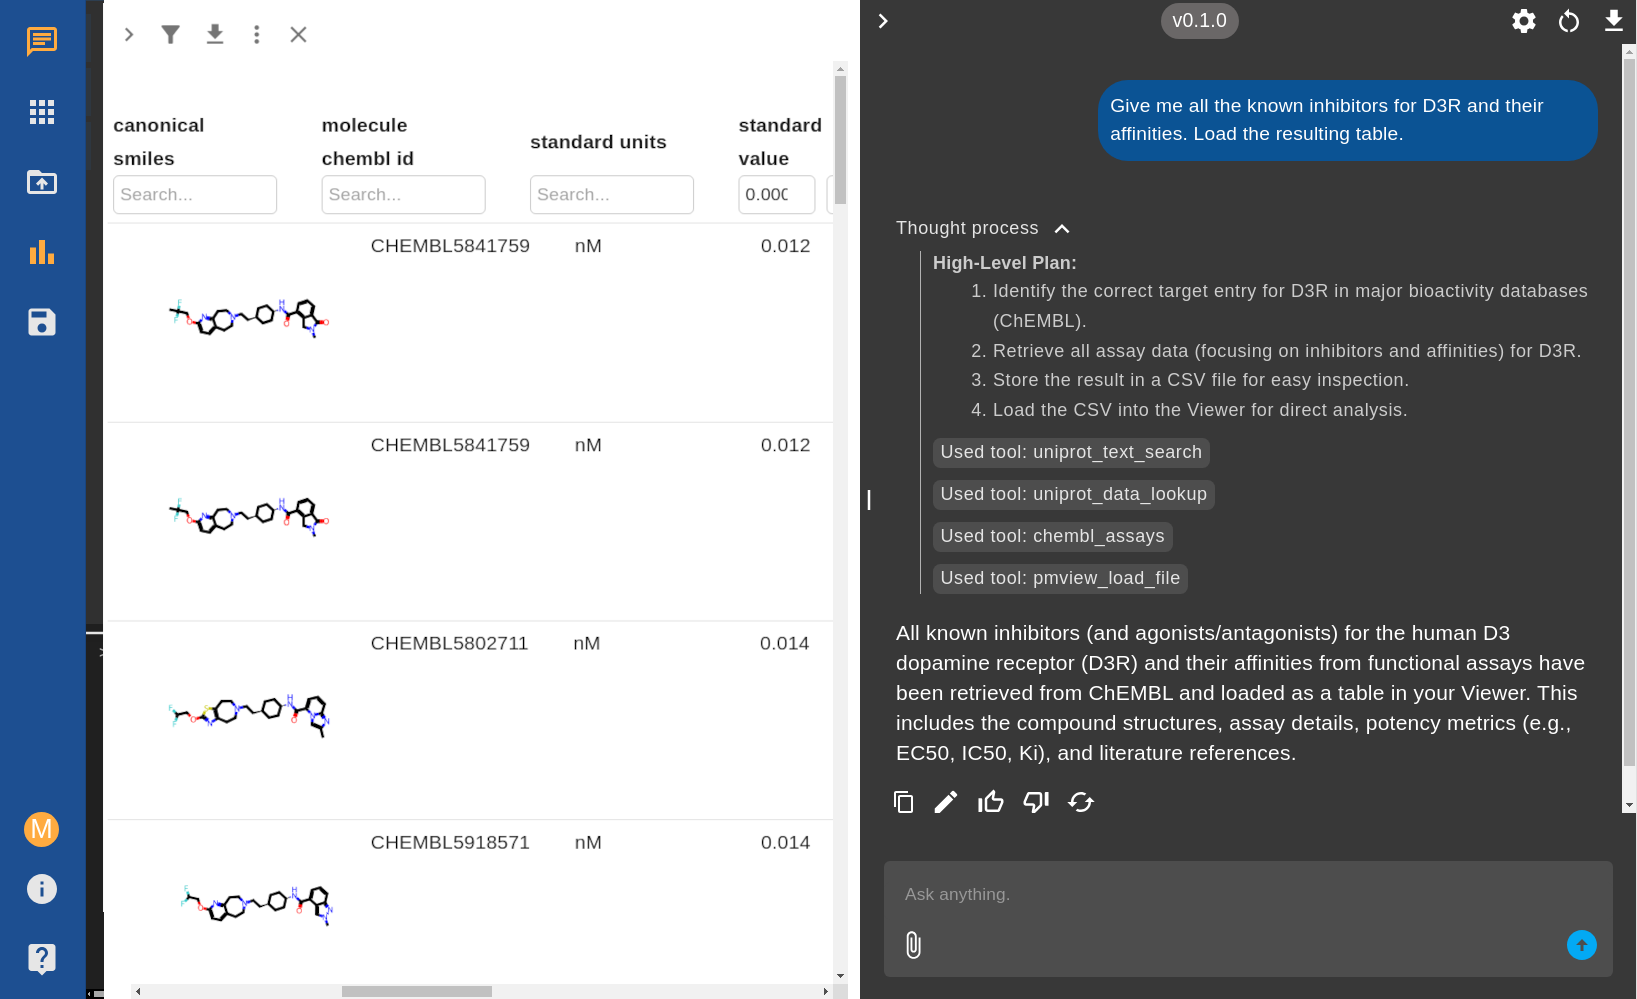
\includegraphics[width=\columnwidth]{Figures/d3r-inhibitors.png}
\caption{
    \textbf{Retrieval and exploration of potent D3R inhibitors.}
    Example user query and system workflow for fetching all known D3R inhibitors and their affinities using \emph{Speak to a Protein}. The chat panel shows the AI's reasoning, including the tools used and the final response. On the left, the interface displays an interactive table of D3R inhibitors, including chemical structures, ChEMBL IDs, assay details, and more, enabling direct exploration and further analysis.}\label{fig:d3r-table}
\end{figure}

In the video trace \url{https://youtu.be/nER3vC90ylQ}, we show how to investigate the differences between the D3 and D2 receptors. The literature search capability can help rapidly surface and synthesize expert knowledge from primary sources to address detailed structural questions.
Upon receiving the prompt \emph{"Based on the literature, compare the binding pockets of D3R and D2R and summarize the main structural features that could be exploited for ligand selectivity."}, the system first uses \emph{UniProt Search} to identify the canonical UniProt IDs for the specified proteins, ensuring precise target selection. Then, using \emph{Literature Search}, an embedding-based literature search is performed, retrieving relevant articles and review information from PubMed Central that address the requested topic.

In this example, the system processed a set of 12 literature passages for D2R and 10 for D3R, selecting at least four distinct, peer-reviewed structural biology studies and related supporting works \citep{Wang2018,Chien2010,Yin2020,Fan2020}. Based on this, the generated answer highlighted that while the orthosteric binding pocket is highly conserved, selectivity can be achieved by targeting differences in the architecture and flexibility of the 'extended binding pocket', as well as in the conformation of extracellular loops. It also described the significance of distinct residues (such as Trp100 and residues in EL1/EL2, positions 1.39 and 7.35) that shape ligand binding modes and selectivity opportunities.
The resulting analysis revealed that while D3R and D2R share a conserved binding pocket core, D2R possesses additional flexible and hydrophobic residues that create a deeper, more accommodating pocket. These structural differences, clearly visualized and annotated in the viewer, help explain how each receptor achieves ligand selectivity, providing actionable insights for targeted drug design.



\subsection{Speaking about the Cyclin-dependent kinase 2}\label{subsec:cdk2}

This case study probes whether \emph{Speak to a Protein} can carry an open-ended drug-discovery question from first principles to a coherent target assessment given a single user prompt. We chose cyclin-dependent kinase 2 (CDK2) \citep{Malumbres2009}, a validated yet contentious oncology target with three decades of structural and bioactivity data, because the breadth of public information makes the difference between a literature recitation and a genuine synthesis observable. The full prompt issued to the agent is reproduced below; no further guidance was provided during the session.

\begin{quote}\itshape
``I want to evaluate CDK2 as a drug-discovery target. Work autonomously and explore the problem thoroughly: begin by forming your own research plan, then execute it step by step. Cover the available structural data, the associated bioactivity, the binding site, and the relevant literature, deciding yourself how best to combine these sources. Use the 3D viewer actively: align and inspect the most informative structures, highlight key binding-site residues and ligand interactions, and capture annotated snapshots you can embed in the final document.

Your goal is to synthesize the evidence into a practical drug-discovery assessment. Identify which CDK2 structures and ligand complexes are most informative, what binding-site features matter for inhibitor design, what potency and selectivity trends are supported by data, what the literature says about CDK2 as a therapeutic target, and what next steps medicinal chemists should consider.

The final report should be easy to follow, visual, and self-contained: reference an annotated 3D image wherever you discuss structural features (residues, pockets, ligand interactions), include the relevant plots, and write clear, well-structured prose suitable to share with medicinal chemists.''
\end{quote}

From this single instruction the agent drafted its own research plan and executed it across four evidence streams. It resolved the canonical human CDK2 entry (UniProt P24941) and retrieved 498 linked PDB structures from RCSB, queried ChEMBL for 3{,}394 single-protein CDK2 activity records together with matched datasets for CDK1, CDK4, CDK6, CDK7, CDK9 and the CDK2/cyclin~E1 and CDK2/cyclin~A2 complexes, and selected representative structures spanning apo, cyclin-bound, orthosteric, allosteric, macrocyclic and ternary degrader states. Those complexes were then loaded in the 3D viewer, aligned, and annotated with snapshots of the cyclin-driven activation transition, the ATP-binding site, and the cyclin~E-dependent interface pocket. The agent finally integrated targeted literature on CDK2 biology, cyclin-E dependency, allosteric chemistry, and degrader strategies, and compiled everything into a self-contained LaTeX report with figures, tables, and references, reproduced verbatim in Appendix~S1.2.

The synthesis reads as a nuanced medicinal-chemistry brief rather than a survey. CDK2 emerges as structurally mature (489 X-ray and 9 cryo-EM entries at median resolution \SI{2.0}{\angstrom}, with 374 explicitly annotated cyclin complexes) and pharmacologically forgiving at the ATP site, where a recurring contact set (Ile10, Ala31, Lys33, the Phe80--Leu83 hinge, Gln131--Asn132, Leu134, Asp145) explains why subnanomolar potency is routine. Selectivity is the binding constraint: across compounds with matched assays the median CDK2 advantage over CDK1 is only 0.32 pChEMBL units, and just 15.3\% achieve a one-log margin, with similar overlap against CDK9. Two structural escape routes from this pan-CDK trap stand out, the ANS allosteric site \citep{betzi2011allosteric} and the more recent cyclin~E-dependent interface pocket exemplified by PDB 8VQ3, and the agent ties them to a biomarker-led therapeutic case (CCNE1-amplified disease, cyclin-E-high tumours, settings of CDK4/6-inhibitor resistance) supported by recent work on replication-stress biology \citep{brown2023forkrepair} and CDK2/cyclin~E heterobifunctional degraders \citep{kwiatkowski2025degrader}. The overall verdict, \emph{``Go, but selectively''}, captures the texture of the recommendation: CDK2 is attractive when biology, modality and a selectivity plan are aligned, and less compelling as a generic pan-cancer kinase project.

Two of the figures the agent generated and embedded in its own report are reproduced in \cref{fig:cdk2_analysis}: an annotated 3D-viewer snapshot of the cyclin~E-dependent allosteric interface pocket and a matched-compound selectivity panel relative to CDK2. They illustrate how the agent interleaved direct structural interpretation with quantitative analysis; the full set of generated figures, tables, and supporting data accompanies the report in the appendix.

\begin{figure}[H]
\centering
\begin{subfigure}[b]{0.38\columnwidth}
    \centering
    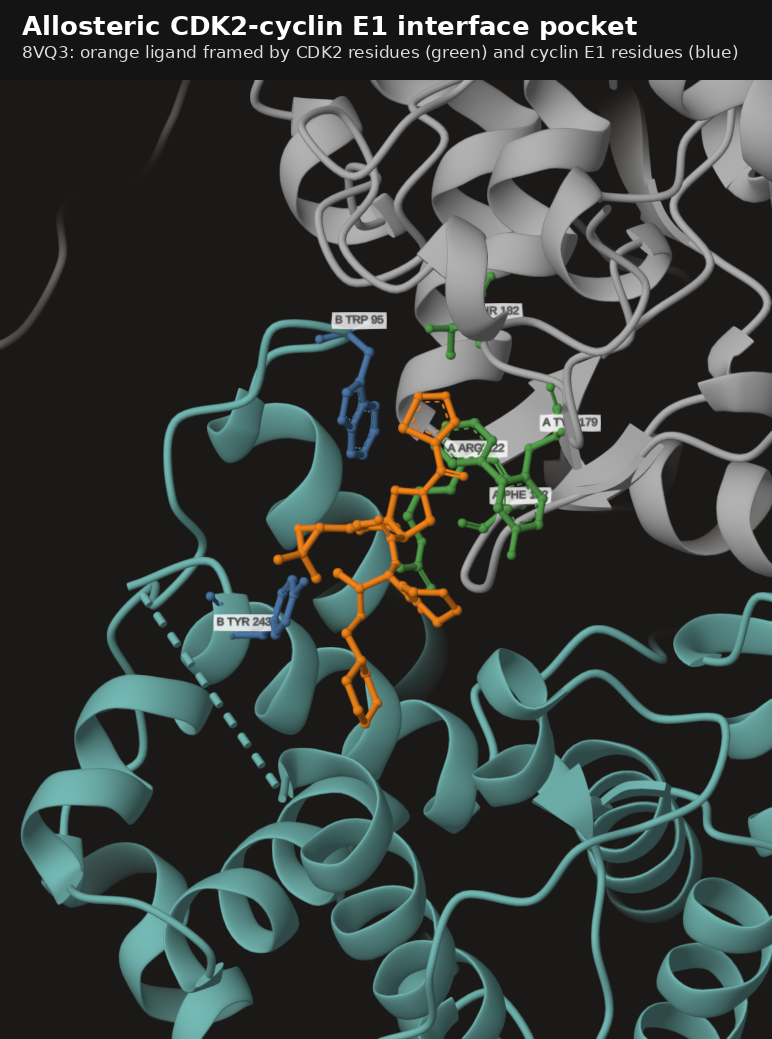
\includegraphics[height=2.6in,keepaspectratio]{Figures/cdk2_viewer_allosteric_interface.png}
    \phantomcaption\label{fig:cdk2_allosteric}
\end{subfigure}\hfill
\begin{subfigure}[b]{0.6\columnwidth}
    \centering
    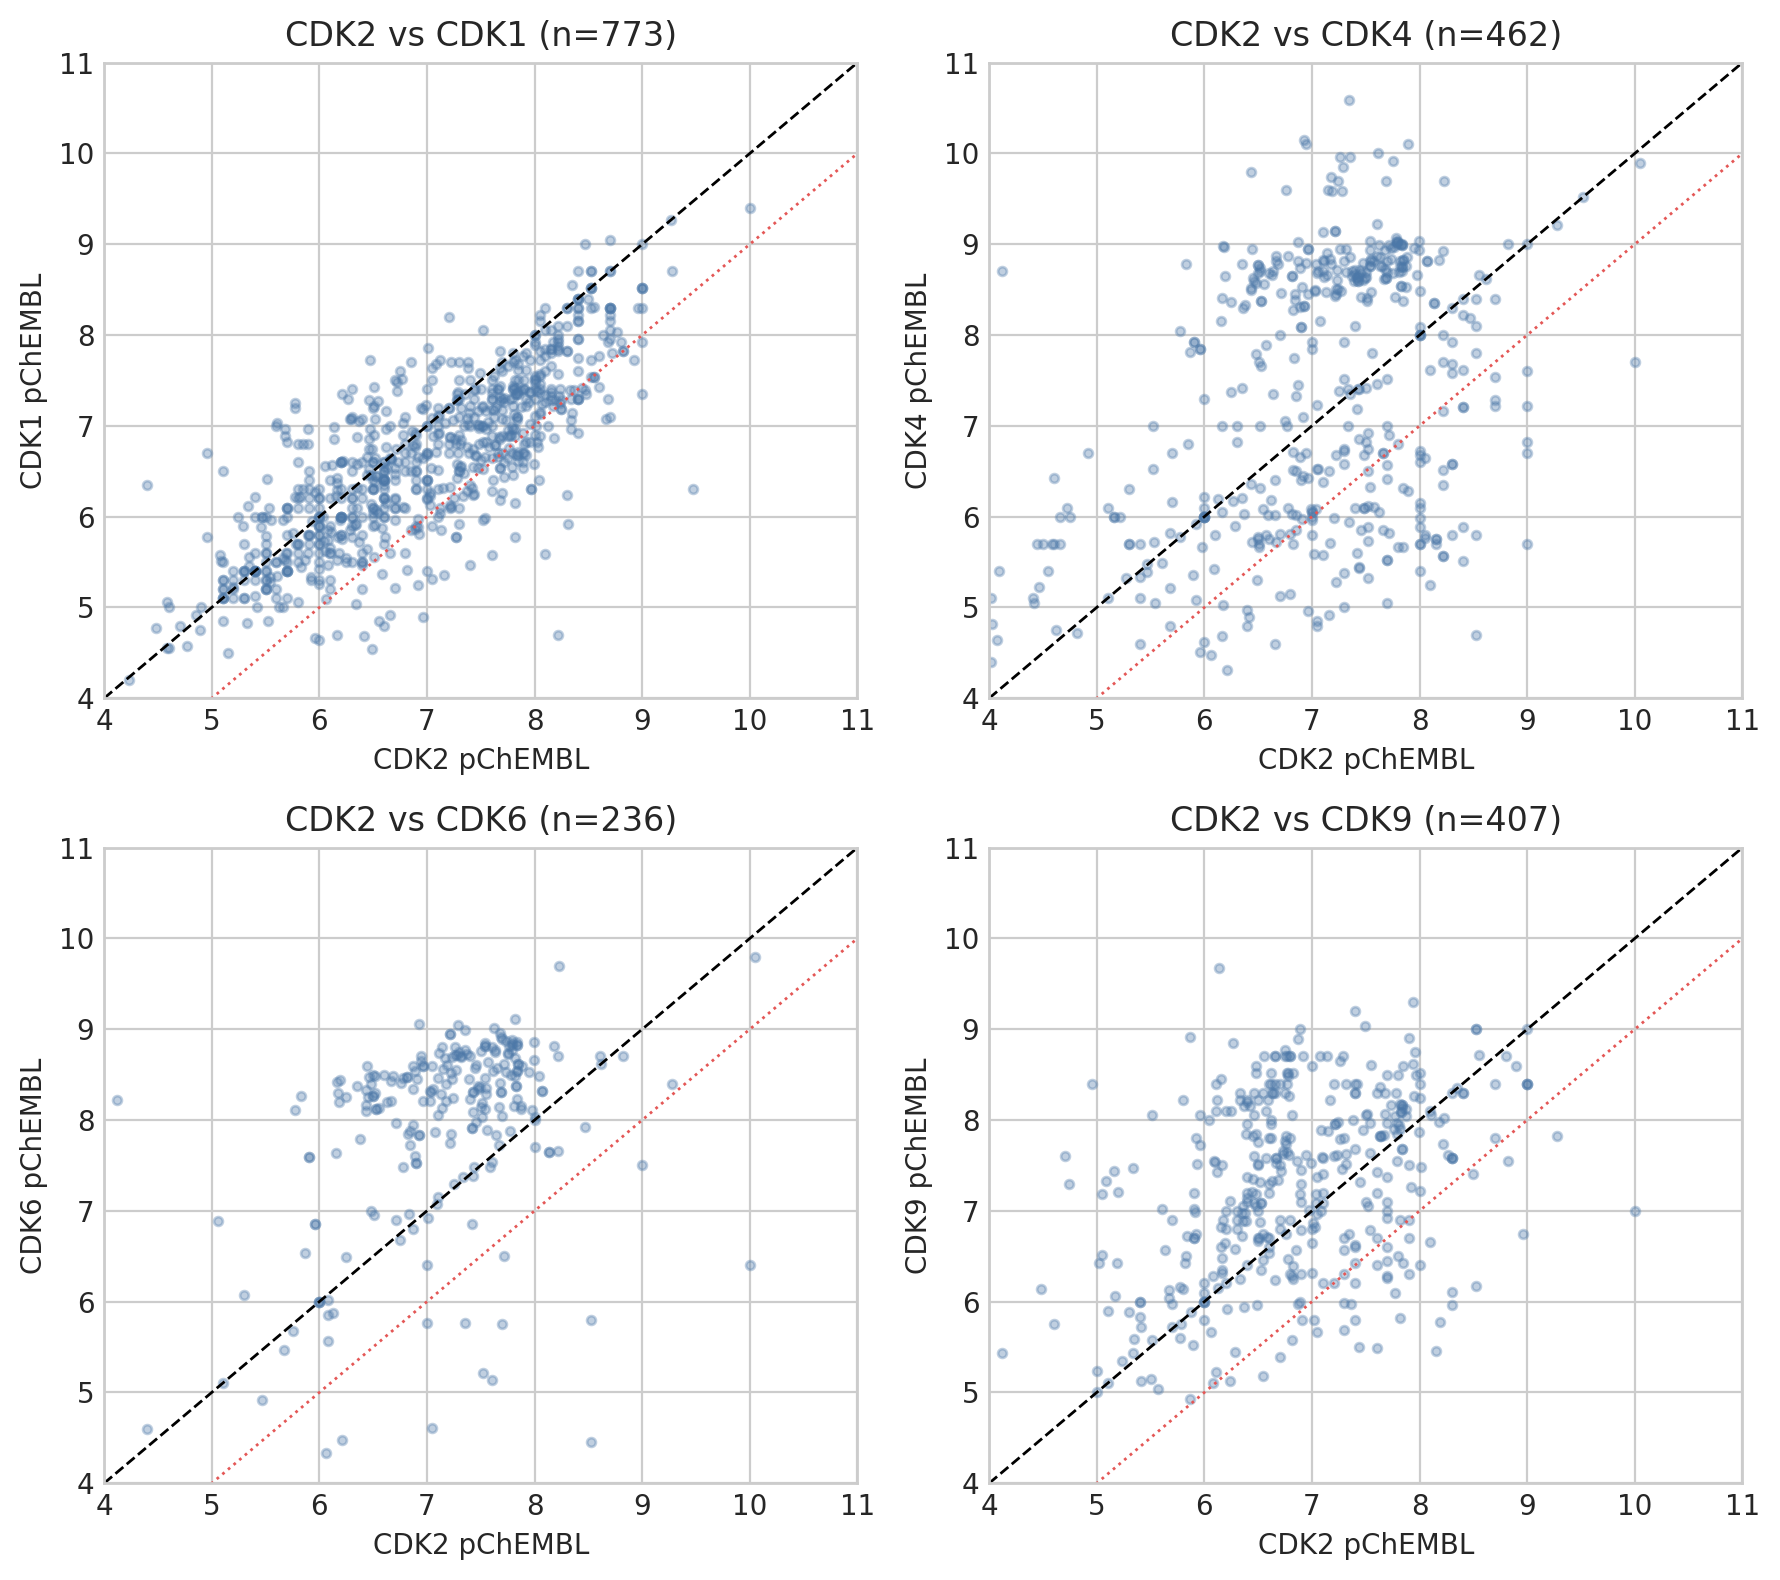
\includegraphics[height=2.6in,keepaspectratio]{Figures/cdk2_selectivity_scatter.png}
    \phantomcaption\label{fig:cdk2_selectivity}
\end{subfigure}
\caption{Two figures the agent generated and embedded in its own report. \textbf{(a)} Annotated 3D-viewer snapshot of the cyclin~E-dependent allosteric interface pocket (PDB 8VQ3), jointly framed by CDK2 (green) and cyclin~E1 (blue) residues, captured by the agent during the analysis. \textbf{(b)} Matched-compound CDK2 selectivity relative to CDK1, CDK4, CDK6, CDK7, and CDK9 from filtered ChEMBL bioactivity; the dashed line is parity, the dotted red line marks a one-log margin in favour of CDK2.}
\label{fig:cdk2_analysis}
\end{figure}

Beyond its conclusions, the run illustrates the working pattern \emph{Speak to a Protein} is designed to enable. One open-ended question produced a connected workflow combining autonomous planning, multi-modal data integration, agentic use of the 3D viewer to capture and reason over annotated structural snapshots, and a publication-ready report, all from a single session. The intermediate artefacts (figures, tables, structured data files, and the report itself) form a queryable knowledge base that the user can carry into downstream conversations, reused as evidence rather than re-derived, closing the loop between question, data, structure, and shareable output inside one interactive session with a scientific co-worker.

\section{Conclusion and Limitations}\label{sec:discussion}

This study demonstrates how \emph{Speak to a Protein} compresses traditional workflows involving several hours of manual data gathering, analysis, and synthesis into an interactive session taking less than an hour. The system's ability to generate publication-ready reports further enhances its utility in collaborative drug discovery environments where rapid understanding and communication of complex structural and biochemical insights are essential for decision-making.

We found the following limitations in the current version of \emph{Speak to a Protein}. The open web application accesses only public information, such as literature, structure-activity relationships, and structural data. This limits the data access and the understanding and downstream calculations. We plan to easily extend it with additional tools to access internal or proprietary datasets, further broadening the scope of information that can be queried and integrated.
 The 3D viewer can experience performance issues when rendering a large number of complex structures simultaneously. We also observe occasional difficulties in seamlessly connecting outputs between tools, stemming from different data representations across the system's components, e.g., residue indices across literature and structural databases. Furthermore, long tool outputs can strain the model's context window. Future work will focus on offloading large data payloads to files and equipping the model with a broader set of tools for file management, allowing for more robust and complex analytical workflows.

\section*{Impact Statement}

This paper presents work whose goal is to advance the field of AI-assisted scientific discovery in structural biology and drug discovery. The system is designed to democratize access to complex protein analysis by enabling researchers without specialized computational skills to perform advanced structural and biochemical analyses. Potential positive impacts include accelerating drug discovery timelines, reducing barriers to entry for bench scientists, and enabling more rapid hypothesis generation in biomedical research. We do not foresee specific negative societal consequences that must be highlighted, as the system operates on publicly available scientific data and is intended to augment, not replace, human scientific judgment.

\bibliography{references}

\end{document}
